\section{はじめに}\label{chap:intro}

電力網の構成制御は,エネルギーの節約や安定した電力供給を支える重要な研
究課題である.
電力網は,高電圧で発電所と変電所を結ぶ\textbf{送電網}と,低電圧で変電
所と家庭や工場といった需要家を結ぶ\textbf{配電網}に分類される.
配電網は変電所と需要家との間で構成される電力供給ネットワークであり,
その構成技術はスマートグリッドや,災害時の障害箇所の迂回構成などを支え
る重要な基盤技術である.

\textbf{配電網問題}は,供給経路に関する\textbf{トポロジ制約}と,電流・
電圧に関する\textbf{電気制約}を満たしつつ,電力の損失を最小にするスイッ
チの開閉状態を求めることが目的である~\cite{Hayashi:dnet:model}.
トポロジ制約は,
短絡(供給経路上のループ,複数の変電所と結ばれる需要家)と
停電(変電所と結ばれない需要家)
が発生しないことを保証する.
電気制約は,供給経路の各区間で許容電流を超えないこと,電気抵抗による電
圧降下が許容範囲を超えないことを保証する.
本稿ではトポロジ制約のみの配電網問題を対象とする.

\begin{figure}[htbp]
o  \centering
%%%%%%%%%%%%%%%%%%%%%%%%%%%%%%%
p  \scalebox{0.7}{%%%%%%%%%%%%%%%%%%%%%%%%%%%%%%%%%%%%%%%%%%%%%%%%%%
% 配電網 例 (第1章で使う)
%%%%%%%%%%%%%%%%%%%%%%%%%%%%%%%%%%%%%%%%%%%%%%%%%%

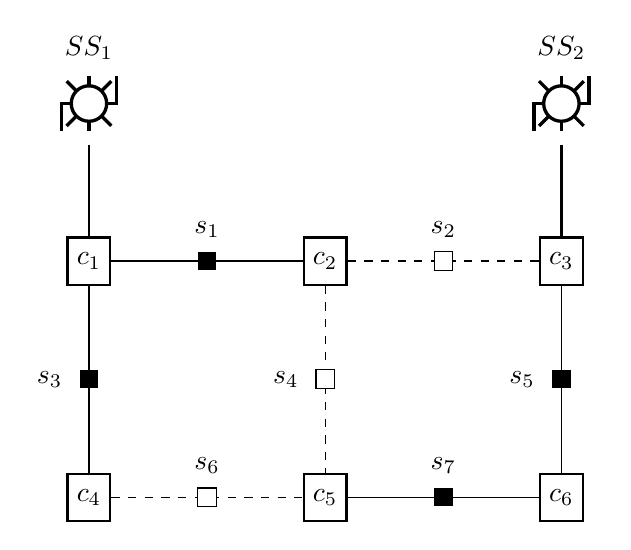
\begin{tikzpicture}

 % 設定
 \tikzset{customer/.style={rectangle,thick,draw=black,minimum height=0.6cm}}
 \tikzset{on_switch/.style={rectangle,fill=black}}
 \tikzset{off_switch/.style={rectangle,draw=black,fill=white}}

 % 補助線
 % \draw [help lines,blue,step=1cm] (-5,0) grid (5,-5);
  
 % substation1 (ホントはnewcommandでできるようにしたかった...)
 \draw [very thick] (-3,0) circle [radius=0.225cm] node[draw=white,minimum size=1cm](root1){};
 \draw [very thick] (-2.775,0)--(-2.65,0)--(-2.65,0.35);
 \draw [very thick] (-3.225,0)--(-3.35,0)--(-3.35,-0.35);
 \draw [very thick] (-3,0.225)--(-3,0.35);
 \draw [very thick] (-3,-0.225)--(-3,-0.35);
 \draw [very thick] [domain=-0.284:-0.159] plot(\x-3,\x);
 \draw [very thick] [domain=0.159:0.284] plot(\x-3,\x);
 \draw [very thick] [domain=-0.284:-0.159] plot(\x-3,-\x);
 \draw [very thick] [domain=0.159:0.284] plot(\x-3,-\x);
 \node at (-3,0.7) {$SS_{1}$};

 % substation2
 \draw [very thick] (3,0) circle [radius=0.225cm] node[draw=white,minimum size=1cm](root2){};
 \draw [very thick] (3.225,0)--(3.35,0)--(3.35,0.35);
 \draw [very thick] (2.775,0)--(2.65,0)--(2.65,-0.35);
 \draw [very thick] (3,0.225)--(3,0.35);
 \draw [very thick] (3,-0.225)--(3,-0.35);
 \draw [very thick] [domain=-0.284:-0.159] plot(\x+3,\x);
 \draw [very thick] [domain=0.159:0.284] plot(\x+3,\x);
 \draw [very thick] [domain=-0.284:-0.159] plot(\x+3,-\x);
 \draw [very thick] [domain=0.159:0.284] plot(\x+3,-\x);
 \node at (3,0.7) {$SS_{2}$};

 % 需要家 customer
 \node[customer] at (-3,-2)(1){$c_1$};
 \node[customer] at (0,-2) (2){$c_2$};
 \node[customer] at (3,-2) (3){$c_3$};
 \node[customer] at (-3,-5) (4){$c_4$};
 \node[customer] at (0,-5) (5){$c_5$};
 \node[customer] at (3,-5) (6){$c_6$};

 % 辺
 % ルート
 \draw [thick] (root1) -- (1);
 \draw [thick] (root2) -- (3);
 % 繋がってない辺は点線
 \foreach \u / \v in {2/3, 2/5, 4/5}
 \draw [dashed] (\u) -- (\v);
 % 繋がってる辺は実線
 \foreach \u / \v in {1/2, 1/4, 3/6, 5/6}
 \draw (\u) -- (\v);

 % スイッチ switch %
 % \node[on_switch] at (-3,-1) (s1){};
 % \node at (-3.5,-1) {$s_1$};
 %
 % \node[on_switch] at (3,-1) (s2){};
 % \node at (2.5,-1) {$s_2$};
 %
 \node[on_switch] at (-1.5,-2) (s1){};
 \node at (-1.5,-1.6) {$s_1$};
 %
 \node[off_switch] at (1.5,-2) (s2){};
 \node at (1.5,-1.6) {$s_2$};
 %
 \node[on_switch] at (-3,-3.5) (s3){};
 \node at (-3.5,-3.5) {$s_3$};
 %
 \node[off_switch] at (0,-3.5) (s4){};
 \node at (-0.5,-3.5) {$s_4$};
 %
 \node[on_switch] at (3,-3.5) (s5){};
 \node at (2.5,-3.5) {$s_5$};
 %
 \node[off_switch] at (-1.5,-5) (s6){};
 \node at (-1.5,-4.6) {$s_6$};
 %
 \node[on_switch] at (1.5,-5) (s7){};
 \node at (1.5,-4.6) {$s_7$};
 %

\end{tikzpicture}

%%%%%%%%%%%%%%%%%%%%%%%%%%%%%%%%%%%%%%%%%%%%%%%%%%%%%%%%%%
%%% Local Variables:
%%% mode: japanese-latex
%%% TeX-master: paper.tex
%%% End:
}
  \caption{配電網問題の例}
  \label{fig:dnet}
\end{figure}
%%%%%%%%%%%%%%%%%%%%%%%%%%%%%%%

% ------------------------------------------
  \thicklines
  \setlength{\unitlength}{1.28pt}
  \small
  \begin{picture}(280,57)(4,-10)
    \put(  0, 20){\dashbox(50,24){\shortstack{根付き全域森\\問題}}}
    \put( 60, 20){\framebox(50,24){変換器}}
    \put(120, 20){\dashbox(50,24){\shortstack{ASPファクト}}}
    \put(120,-10){\alert{\bf\dashbox(50,24){\scriptsize{\shortstack{ASP符号化\\(論理プログラム)}}}}}
    \put(180, 20){\framebox(50,24){ASPシステム}}
    \put(240, 20){\dashbox(50,24){\shortstack{根付き全域森\\問題の解}}}
    \put( 50, 32){\vector(1,0){10}}
    \put(110, 32){\vector(1,0){10}}
    \put(170, 32){\vector(1,0){10}}
    \put(230, 32){\vector(1,0){10}}
    \put(170, +2){\line(1,0){4}}
    \put(174, +2){\line(0,1){30}}
  \end{picture}  

% ------------------------------------------

トポロジ制約のみの配電網問題の例を図\ref{fig:dnet}に示す.
この例は,
2つの変電所$\{SS_{1}, SS_{2}\}$,
7個のスイッチ$\{s_{1},\ldots, s_{7}\}$,
6つの需要家$\{c_{1},\ldots, c_{6}\}$
から構成されている.
$\blacksquare$は閉じたスイッチ,
$\square$は開いたスイッチを表している.
配電網問題の実行可能解は閉じたスイッチの集合で表すことができる.
この例は実行可能解$\{s_{1},s_{3},s_{5},s_{7}\}$を表している.
需要家$\{c_{1},c_{2},c_{4}\}$は変電所$SS_{1}$から,
需要家$\{c_{3},c_{5},c_{6}\}$は変電所$SS_{2}$から電力を供給され,
トポロジ制約を満たしていることがわかる.

配電網問題は求解困難な組合せ最適化問題の一種であり,
これまでフロンティア法を用いた解法等が提案されている~\cite{Minato:dnet:ZDD}.
トポロジ制約のみの配電網問題は,与えられた連結グラフと根と呼ばれる特殊
なノードから,\textbf{根付き全域森}を求める部分グラフ探索問題に帰着で
きることが知られている~\cite{Minato:dnet:netuki}.
以降,この問題を\textbf{根付き全域森問題}と呼ぶ.

\textbf{解集合プログラミング}(Answer Set Programing; ASP\cite{%
  Baral03:cambridge,%
  Gelfond88:iclp,%
  Inoue08:jssst,%
  Niemela99:amai})は,
論理プログラミングから派生したプログラミングパラダイムである.
ASP言語は,一階論理に基づく知識表現言語の一種であり,
論理プログラムはASPのルールの有限集合である.
ASPシステムは論理プログラムから安定モデル意味論~\cite{Gelfond88:iclp}
に基づく解集合を計算するシステムである.
近年,SATソルバーの技術を応用した高速なASPシステムが確立され,
制約充足問題,プランニング,システム生物学,時間割問題,システム検証な
ど様々な分野への実用的応用が急速に拡大している~\cite{ASPAISAT}.

本稿では,解集合プログラミングを用いた根付き全域森問題の解法につ
いて述べる.提案アプローチでは,まず与えられた問題インスタンスをASPの
ファクト形式に変換した後,それらファクトと根付き全域森問題を解くための
ASP符号化と結合した上で,高速ASPシステムを用いて解を求める
(図~\ref{fig:arch}参照).

根付き全域森問題を解くASP符号化(論理プログラム)として,
基本符号化と改良符号化の2種類を考案した.
% 両符号化は,根付き全域森問題の制約を7個程度のASPルールで簡潔に表現できる.
% 基本符号化は,根付き全域森の根付き連結制約を
% at-least-one制約とat-most-one制約で表現した基本的な符号化に対し,
特に,改良符号化は,根付き全域森問題の連結制約をASPの個数制約で表現す
ることにより,基礎化後のルール数を少なく抑えるよう工夫されており,
大規模な問題に対する有効性が期待できる.

%%%%%%
また,配電網における障害時の復旧予測への応用を狙いとし,
根付き全域森問題の2つの実行可能解が,局所的な変形による遷移だけで互い
に移りあえるかを問う``解の遷移問題''への拡張を行なった.
% ある初期配電網の構成からスタートして,
% トポロジ制約を満たした上で,一度に切り替えるスイッチの数を$k$個以下に制限し,
% 最終的に目的とする配電網の構成を得るためのスイッチの切り替え手順を求める遷移問題
% への拡張を行い,
この遷移問題を解くには,複数の根付き全域森問題を繰り返し解く必要がある.
しかし,各問題中の制約の大部分は共通であるため,ASP システムが同一の
探索空間を何度も調べることになり,求解効率が低下するという問題点がある.
この問題を解決するために,マルチショットASP解法を用いた実装を提案する.
この解法は,ASPシステムが同様の探索失敗を避けるために獲得した学習節を
(部分的に)保持することで,無駄な探索を行うことなく,制約を追加した論理
プログラムを連続的に解くことができる.そのため,求解性能の向上が期待できる.
% 解を探索するための手法として,外部プログラムによって繰り返しASPシステム
% を呼び出し探索する手法と,ASPシステム\clingo のライブラリを利用した探索手法を考案した.
% ライブラリを利用することで,ASPシステムの呼び出しが1回で済むため,起動時のオーバヘッドの
% 短縮につながり,高速に解が得られると期待できる.また,探索の中で部分的に学習節を共有
% できるため,高速化につながると期待できる.

提案アプローチの有効性を評価するために,
DNET (Power Distribution Network Evaluation Tool)~\footnote{%
\url{https://github.com/takemaru/dnet}}
に公開されている問題集と,
Graph Coloring and its Generalizations~\footnote{%
\url{https://mat.tepper.cmu.edu/COLOR04/}}
に公開されているグラフ彩色問題を元に生成した根付き全域森問題を用いて,
実行実験を行なった.
その結果,改良符号化は,基本符号化と比較して,より多くの問題をより高速
に解くことができた.
また,改良符号化は辺数(スイッチ数)が40,000個を超える問題も解いており,
大規模問題に対するASPの有効性が確認できた.

\comment{遷移問題の実験結果についても簡単に書いてはどうですか?}
%
解の遷移問題に対する実験では,DNETで公開されている実用規模の問題をベース
として作成したベンチマークを用いて,シングルショット符号化とマルチショット符号化
の比較実験を行った.その結果,マルチショット符号化は,シングルショット符号化と
比較して,すべての問題をより高速に解くことができた.平均で3.3倍の高速化を実現しており,
マルチショットASP解法の優位性が確認できた.


本稿の構成は以下の通りである.
\ref{chap:problem}節で根付き全域森の定義を示し,
\ref{chap:asp}節で解集合プログラミングの説明を行う.
\ref{chap:encode}節で根付き全域森問題のASP符号化を示し,
\ref{chap:trans}節で根付き全域森問題の遷移問題への拡張を行う.
\ref{chap:exp}節で評価実験とその考察を述べ,最後に,
\ref{chap:conc}節で本稿をまとめる.

%%% Local Variables:
%%% mode: japanese-latex
%%% TeX-master: "paper"
%%% End:
